\chapter{ESC characterization}
This section will introduce the different experiments realized to characterize the ESC input-output behavior. For all of them, the real-time data was recorded using the "logger" provided in PX4 that allows to store topics in the SD card connected to the circuit board. The topics logged were:
\begin{itemize}
	\item "actuator\_controls\_0", to see the control signal send to the ESCs.
	\item "esc\_status", to check the rotor speed RPM.
	\item "adc\_report" to read the current sensor analog signal.
\end{itemize}

\section{Sensing Evaluation}
The purpose of this experiment is to determine the quality of the measurements that the ESC provides. The focus is on rotor speed measurements and current sensing. For both experiments in this section (rpm and current sensor validation), a staircase throttle signal was sent and the steady state values were used. Figure \ref{fig:sensing_validation} shows typical experiment data for this section.

\begin{figure} 
    \centering
    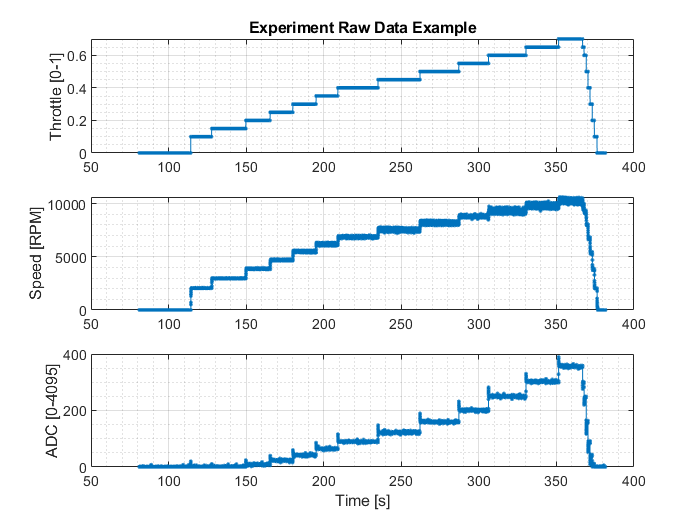
\includegraphics[width=0.6\textwidth]{images/experiment_sample_data.png}
    \caption{Sensing Validation Experiment Example}
    \label{fig:sensing_validation}
\end{figure}

\subsection{ESC RPM feedback}
Experiment in the figure above was repeated 7 times to obtain more data. Here, the rotor speed was measured using the manual tachometer and comparing it to the RPM measurements coming from the ESC. Figure \ref{fig:rpm_validation} shows this relationship. There is very high accuracy and a strong linear behavior. For instance, the fitted curve is characterized as in \ref{eq:rpm_validation}. Notice the high $R^2$ value and slope of $1$. Accordingly, the average relative error is $0.6366\%$

\begin{equation}
  RPM_{actual} = 1.0064RPM_{ESC}-1.523 \quad with \quad R^2=0.999\, .
    \label{eq:rpm_validation}
\end{equation}

\begin{figure} 
    \centering
    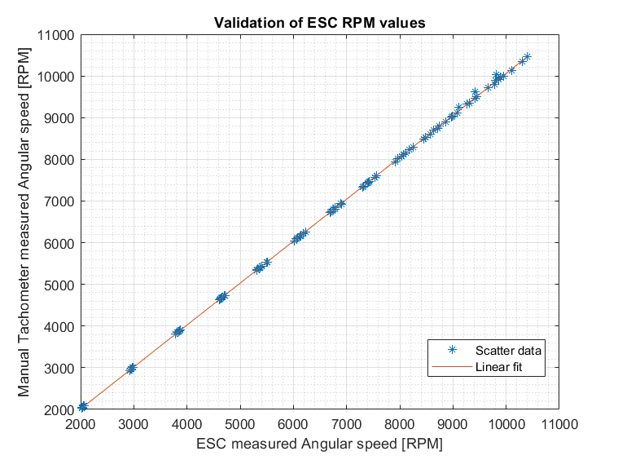
\includegraphics[width=0.6\textwidth]{images/rpm_validation.png}
    \caption{Validation of RPM measurements}
    \label{fig:rpm_validation}
\end{figure}

Therefore, the RPM measurement is accurate enough to be used for feedback control purposes. The accuracy is expected to be high because the ESC needs to have angular estimates of the rotor positioning in order to run and rotor speed is internally calculated by counting revolutions in a fixed period.

\subsection{ESC current sensing}
Another important sensor, to calculate power consumption and in the future help estimate time of flight more accurately is the current sensor. 
\newline

There are two trends to send this information: digitally via an element in the Dshot packet or analogically. In both cases, the the measurement is done via a shunt resistor and the voltage across it will be measured with an ADC. In the digital case, the ADC is located in the ESC and therefore the current estimation is calibrated with the nominal shunt-resistor value. In the analog case, the ADC needs to be in the flight controller. These shunt resistors are usually of $5\%$ tolerance, hence the current measurements need to be calibrated accordingly. This is impossible in the digital case if the firmware is closed-source.\\

As the measurement is shunt resistor based, it is expected that the relationship is highly linear. This is confirmed in Figure \ref{fig:current_validation} that was used to calibrate the current sensor measurement. 
\begin{figure} 
    \centering
    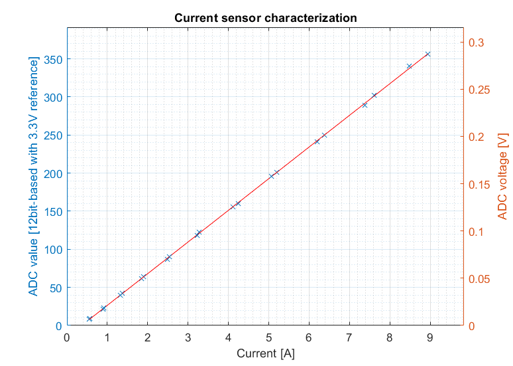
\includegraphics[width=0.6\textwidth]{images/current_validation.png}
    \caption{Validation of current measurements}
    \label{fig:current_validation}
\end{figure}

\section{Motor-drive dynamics}

\subsection{RPM-Voltage-Throttle relation}
As shown in previous literature, the rotor speed also varies with respect to battery voltage. Therefore, an experiment similar to the one described in Figure \ref{fig:sensing_validation} was set up for different battery voltages that were varied using a power supply. After analyzing the data, one can see that even though the voltage does not change the output as dramatically as throttle does, the variation is significant for instance it appears linear when looking at the cross-section. It is also coherent with theory as higher voltages generate linearly related higher currents and therefore higher induced magnetic field. In the end allowing for higher torques and steady state rotor speed.
Furthermore, a significant non-linearity can be observed in the dependence from throttle. The reason for this is the way the ESC approximates driving voltages (switching transistors) because it introduces high frequency current components that can pass through parasitic capacitances in the circuit. Therefore, augmenting from the linear throttle dependency model explained in \cite{Moutinho2015}, the quadratic model in Equation \ref{eq:rmp_V_throt_quad} is introduced to account for non-linearities. The parameters were found using Non-linear least squares optimization method given the test data.
\begin{equation}
\begin{split}
 \omega &= (at^2 +bt+c)V\, .\\
 a&=-7.038\times 10^{-5}\\
 b&=0.4155\\
 c&=3.168
\end{split} 
\label{eq:rmp_V_throt_quad}   
\end{equation}

Figure \ref{fig:rpm_fit} shows the data points as black dots and the surface represents the model proposed above. The fit provided a good approximation with $R^2=0.996$ and on average $1.5\%$ error in rotor speed obtained.

\begin{figure} 
    \centering
    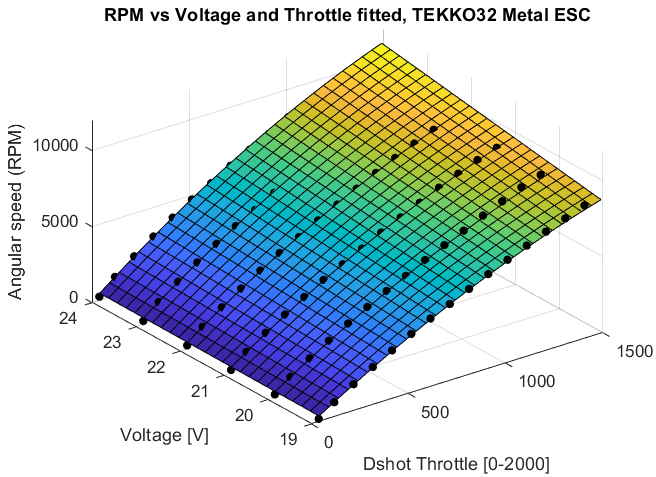
\includegraphics[width=0.65\textwidth]{images/surf_rpm_model.png}
    \caption{RPM dependence on throttle and voltage}
    \label{fig:rpm_fit}
\end{figure}



\subsection{ESC to ESC discrepancies}
Given the complexity of the OMAV and that the current control assumes equal throttle to RPM mapping for all ESCs, this investigation also assessed the  variability in rotor speed depending on the hardware used. To do so, different ESC-motor combinations were subject to staircase-like signals as in the previous experiments. Two factors were considered into this analysis: motors and ESCs. Indeed, significant variations for different motors and ESCs combinations were found as it is summarized in Figure \ref{fig:esc_dis_all_rpm} and \ref{fig:esc_dis_all_thrust}.\\

\begin{figure}[!tbp]
  \centering
  \makebox[\textwidth]{
  \subfloat[RPM]{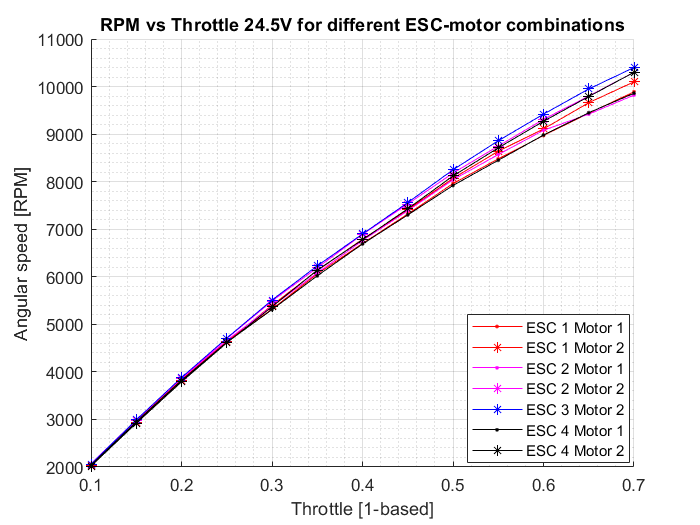
\includegraphics[width=0.65\textwidth]{images/esc_dis_all_rpm.png}\label{fig:esc_dis_all_rpm}}
  \hfill
  \subfloat[Thrust]{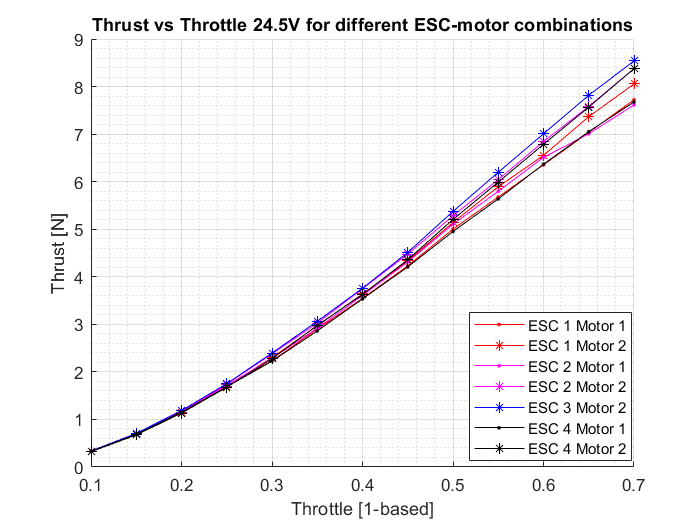
\includegraphics[width=0.65\textwidth]{images/esc_dis_all_thrust.png}\label{fig:esc_dis_all_thrust}}
  }
  \caption{Discrepancies for different ESC-motor discrepancies
  \label{fig:esc_discrepancies_overall}}
\end{figure}

From Figure \ref{fig:esc_discrepancies_overall}, we can see that variations between same-model parts can cause discrepancies of $5\%$ in rotor speed and $10\%$ in thrust generated. Therefore, calibration is key. Additionally, Figure \ref{fig:esc_mot_stats} shows the representation of these measurements as Gaussian random variables with the the mean and double standard deviation range (for $95\%$ confidence interval). Note that the standard deviation increases with throttle too. With this model, the variability range for rotor speed was was up to $1.5N$ and $960RPM$ at high throttle. Two of the factors that could cause this variation were isolated and tested separately, to see individual contributions to uncertainty. That is, testing with different motors for a fixed ESC and vice versa. 



\begin{figure}[!tbp]
  \centering
  \makebox[\textwidth]{
  \subfloat{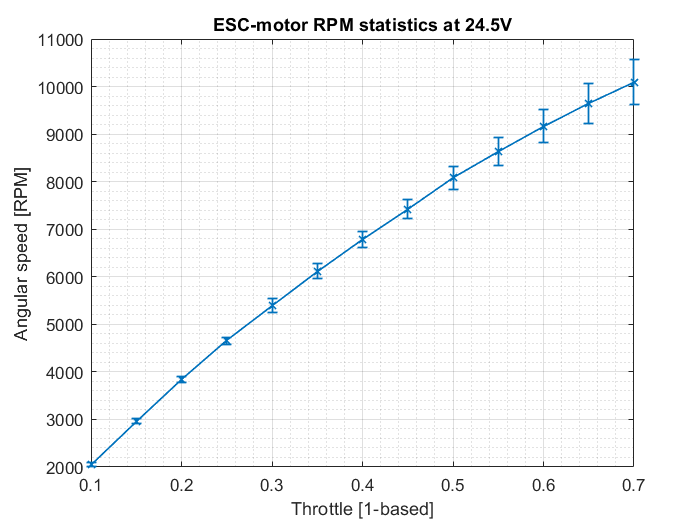
\includegraphics[width=0.6\textwidth]{images/esc_mot_stats_rpm.png}}
  \hfill
  \subfloat{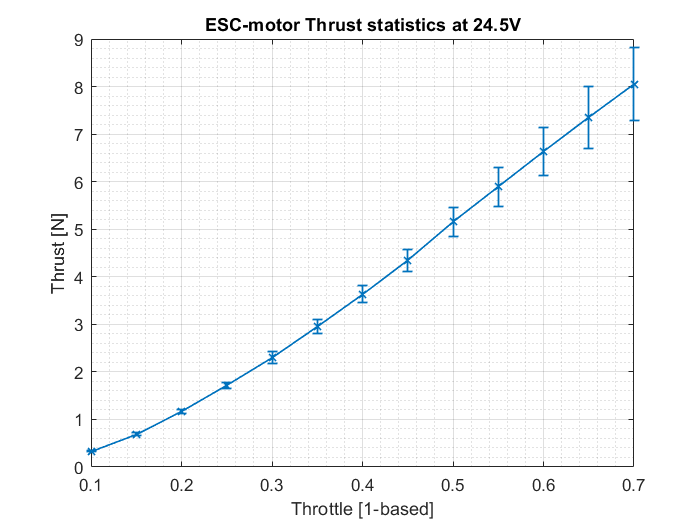
\includegraphics[width=0.6\textwidth]{images/esc_mot_stats_thrust.png}}
  }
  \caption{ESC-motor combination characterization showing mean and 2 standard deviation range}
  \label{fig:esc_mot_stats}
\end{figure}

\subsubsection{Motor differences}
For this analysis, the experiments with the same ESC but different motor were analyzed. A typical curve analyzed in this section is shown in Figure \ref{fig:mot_discr}. Again, the difference between the response with two motors increases with throttle, reaching a $440RPM$ difference at 0.7 throttle. \\

Higher rotor speed values accentuate this difference more that lower ones. This suggests that a viscous friction element acting differently since the same propeller is used. The reason to suggest viscous friction are the ball bearings. In fact, \cite{Armstrong-H1994} studied friction for robotic machines, where bearings are explained to have a representative viscous friction component.\\

Another element contributing to higher viscous friction would be slight miss-alignments when manufacturing the motors. That is, axis-bearing misalignments that would result bearing load increase , which in turn rises friction torque.


\begin{figure} 
    \centering
    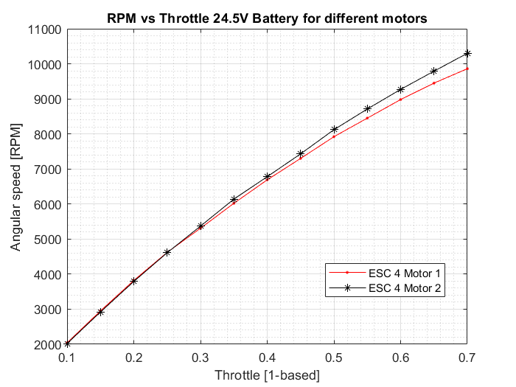
\includegraphics[width=0.65\textwidth]{images/motor_discrepancy.png}
    \caption{Impact of using different motors}
    \label{fig:mot_discr}
\end{figure}


\subsubsection{ESC differences}

\begin{figure} 
    \centering
    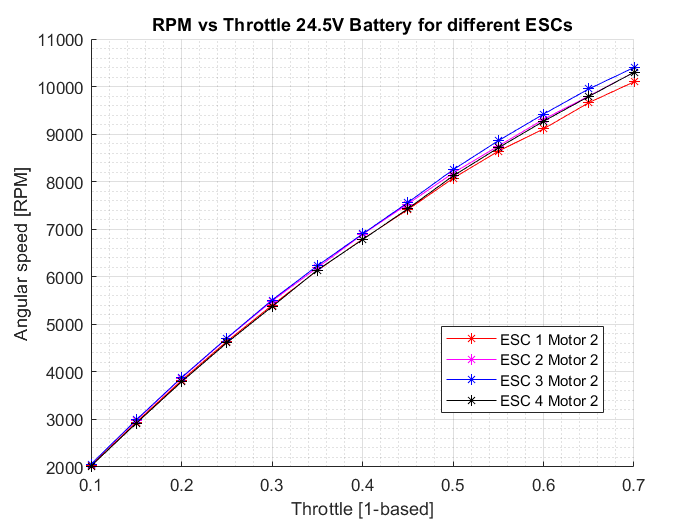
\includegraphics[width=0.65\textwidth]{images/esc_discrepancy.png}
    \caption{Impact of different ESCs}
    \label{fig:esc_discr}
\end{figure}

\subsection{Transient response and active break}
\subsection{Coaxial rotor interference}


\section{Frequency Modulation and Efficiency}
